\section{Preliminaries}

\subsection{A discrete grid of robots}

% WORKSPACE 
Let our grid-based workspace be modeled as a graph \( G \coloneqq (V, E)\). 
Let it be a rectangle \(n_1 \times n_2\) where \(n_1, n_2 \geq 2 \text{ and } n_1, n_2 \in \mathbb{N}\). 
Define the vertices as \(V \coloneqq \set{1, 2, \dots , n_1} \times \set{1, 2, \dots , n_2}\).
For any \(v \in V\), let \(v_x, v_y\) be such that \(v = (v_x, v_y)\). 
We will call \(v_x\) the \(x\)-coordinate of \(v\), and \(v_y\) its \(y\)-coordinate.
To measure distance, we use the \emph{Manhattan norm} \(L_1 = \manhattan{v - w} \coloneqq (\abs{v_x - w_x} + \abs{v_y - w_y})\). Using this, the edges can be defined as \(E = \set{(v, w) \mid \manhattan{v - w} = 1 \text{ for } v, w \in V}\). In other words, nodes are only connected to their up to four immediate neighbors in the grid.

% ROBOTS AND CONFIGURATIONS
Let there be \(N \leq \nngrid\)  robots in our workspace. 
We can identify them by a number \(r \in R := \set{1, 2, \dots , N} \subset \mathbb{N}\). 
Let \(\bot\) represent the empty vertices.
A \emph{configuration} is then a mapping \(\conf{} : V \mapsto \set{1, 2, \dots, N, \bot}\) injective upon the robots in \(R\). 
Injectivity implies no two vertices in \(V\) can be occupied at once, so there will always be exactly \((\nngrid - N)\) empty squares in the grid.

% CONFIGURATION INVERSE
The \emph{inverse} of a configuration \(\iconf{}{r} = (x, y), \; r \in R\), is another function mapping robots to their respective positions.
The robots move synchronously and in parallel, up to a single edge at a time. 
A valid (no-collision) configuration \(\conf{1}\) can thus be \emph{transformed} into another valid configuration \(\conf{2}\) in a \emph{single step} if and only if:

% TRANSFORMATION REQUIREMENTS
\begin{align}
	& \parens{\iconf{1}{r} = \iconf{2}{r} \lor (\iconf{1}{r}, \iconf{2}{r}) \in E, \; \forall r \in R}\label{req:limited_movement}\\
	\land & \parens{\nconf{1}{v} = \nconf{2}{w} \Rightarrow \nconf{2}{v} \neq \nconf{1}{w}, \; \forall v, w \in V}\label{req:no_swaps}
\end{align}

In other words, \cref{req:limited_movement} means a robot can stay in place or move to a neighboring square at every step, while \cref{req:no_swaps} forbids two robots from swapping places in a single transformation step (and they can never occupy the same vertex), equivalent to a collision in the real world.

% SCHEDULE
Denote a single transformation step by \(\conf{i} \rightarrow \conf{i + 1}\). 
A \emph{schedule} is a sequence of transformation steps \(S \coloneqq \conf{1} \rightarrow \conf{2} \rightarrow \cdots \rightarrow \conf{k}\). 
A configuration \(\conf{s}\) can be transformed into a configuration \(\conf{t}\) if there exists a schedule \(\conf{s} \rightarrow \conf{s + 1} \rightarrow \cdots \rightarrow \conf{t - 1} \rightarrow \conf{t}\).

% PROBLEM DEFINITION
\begin{definition}\label{def:motion_planning_problem}
	Given a start configuration \(\conf{s}\) and a target configuration \(\conf{t}\) of a workspace, the \emph{motion planning problem} asks to find a schedule that transforms \(\conf{s}\) into \(\conf{t}\).
\end{definition}

Denote the tuple of a workspace and two configurations \(I \coloneqq \parens{G,\ \conf{s},\ \conf{t}}\) as a problem \emph{instance}. 

\begin{remark}\label{remark:reachability}
	For a \(2 \times 2\) square and any \(1 \times n\) rectangle, where \(n \geq 2\), there exist pairs of configurations that are not reachable from each other via any schedule. 
	See \cref{fig:reachability} for an example. For any other rectangular workspace there always exists such a schedule. 
\end{remark}

% IMPOSSIBLE 2*2 SQUARE FIGURE
\begin{figure}[h]
	\centering
	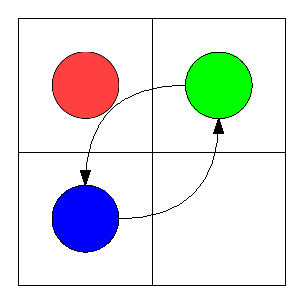
\includegraphics[width=4cm]{include/impossible_2x2.eps}
	\caption{A minimal example of an unsolvable motion planning problem: there exists no valid schedule which swaps the green and blue robots.}\label{fig:reachability}
\end{figure}

% MAKESPAN
\begin{definition}\label{def:makespan}
	The number of single transformation steps in a schedule is called the \emph{makespan} of that schedule.
\end{definition}

\begin{definition}\label{def:optimality}
	Let \(\schedules\) denote the set of all valid schedules for some problem instance \(I\). 
	A schedule \(S_\text{opt}\) is \emph{optimal} with respect to some cost function \(f : \schedules \mapsto \mathbb{N}\) mapping all valid schedules to some integer value if and only if \(f(S) \geq f(\sopt)\) for all such valid schedules \(S \in \schedules\).
\end{definition}

% M3PP -- MINIMUM MAKESPAN MOTION PLANNING PROBLEM
\begin{definition}\label{def:m3pp}
	Let the makespan of a schedule be such a cost function: \(M : S \mapsto \parens{\text{number of steps in S}}\). 
	The \emph{minimum makespan motion planning problem} asks to find an \emph{optimal} schedule with respect to the makespan \(M\) for some input problem instance.
\end{definition}

\begin{remark}
	The \emph{minimum makespan} for any motion planning problem instance \(I \coloneqq \parens{G,\ \conf{s},\ \conf{t}}\) is bounded below by \(\max(\set{\manhattan{\iconf{s}{r}, \; \iconf{t}{r}}, \; r \in R})\).
\end{remark}

\begin{definition}
	Let the aforementioned lower bound to a schedule with makespan \(M\) be denoted by \(L\). 
	The \(\emph{stretch factor}\) for that schedule is then defined as \(\frac{M}{L}\), which is always at least 1. 
\end{definition}

\subsection{Some general notation}

\begin{definition}
	A function \(f(n)\) has an asymptotic upper bound \(g(n)\) if there are some constants \(c \text{ and } n_0\) such that \(f(n) \leq c\cdot g(n),\ \forall n \geq n_0\). 
	It is then denoted as \(f(n) = \mathcal{O}(g(n))\). 
\end{definition}

% Let \emph{A} be some algorithm. 
% \fda{\(A\) is said to run in \emph{polynomial time} ... if the execution of \(A\) by a deterministic Turing machine is done in a polynomial number of steps w.r.t.\ the input bit length... (are yyou sure you want do define this? I think is better to assume it is known)}
% It is \emph{polynomial time} and often said to be \emph{efficient} if the runtime of \emph{A} is bounded by some polynomial function \(T(A) = O(n^c)\) for some constant \(c\).

Let OPT be the optimal (minimum) value of some function \(f\). 
If some algorithm \(A\) can always find a solution that maps to within a \(\rho\)-factor of the optimal value: \(OPT \leq f(x_A) \leq \rho \cdot OPT\), the algorithm is called a \(\rho\)-approximation algorithm. 
